\section{Puppet Run}

In this section we are going to explain what is a Puppet run: how Puppet
determines how to configure a machine following the service manages
instructions. It is important to remember that all the machines in the
system have their hostgroup and environment registered in Foreman: this
allows Puppet to understand which configuration they should have.

The diagram below summarises the main interactions of a Puppet run:

\begin{figure}[H]
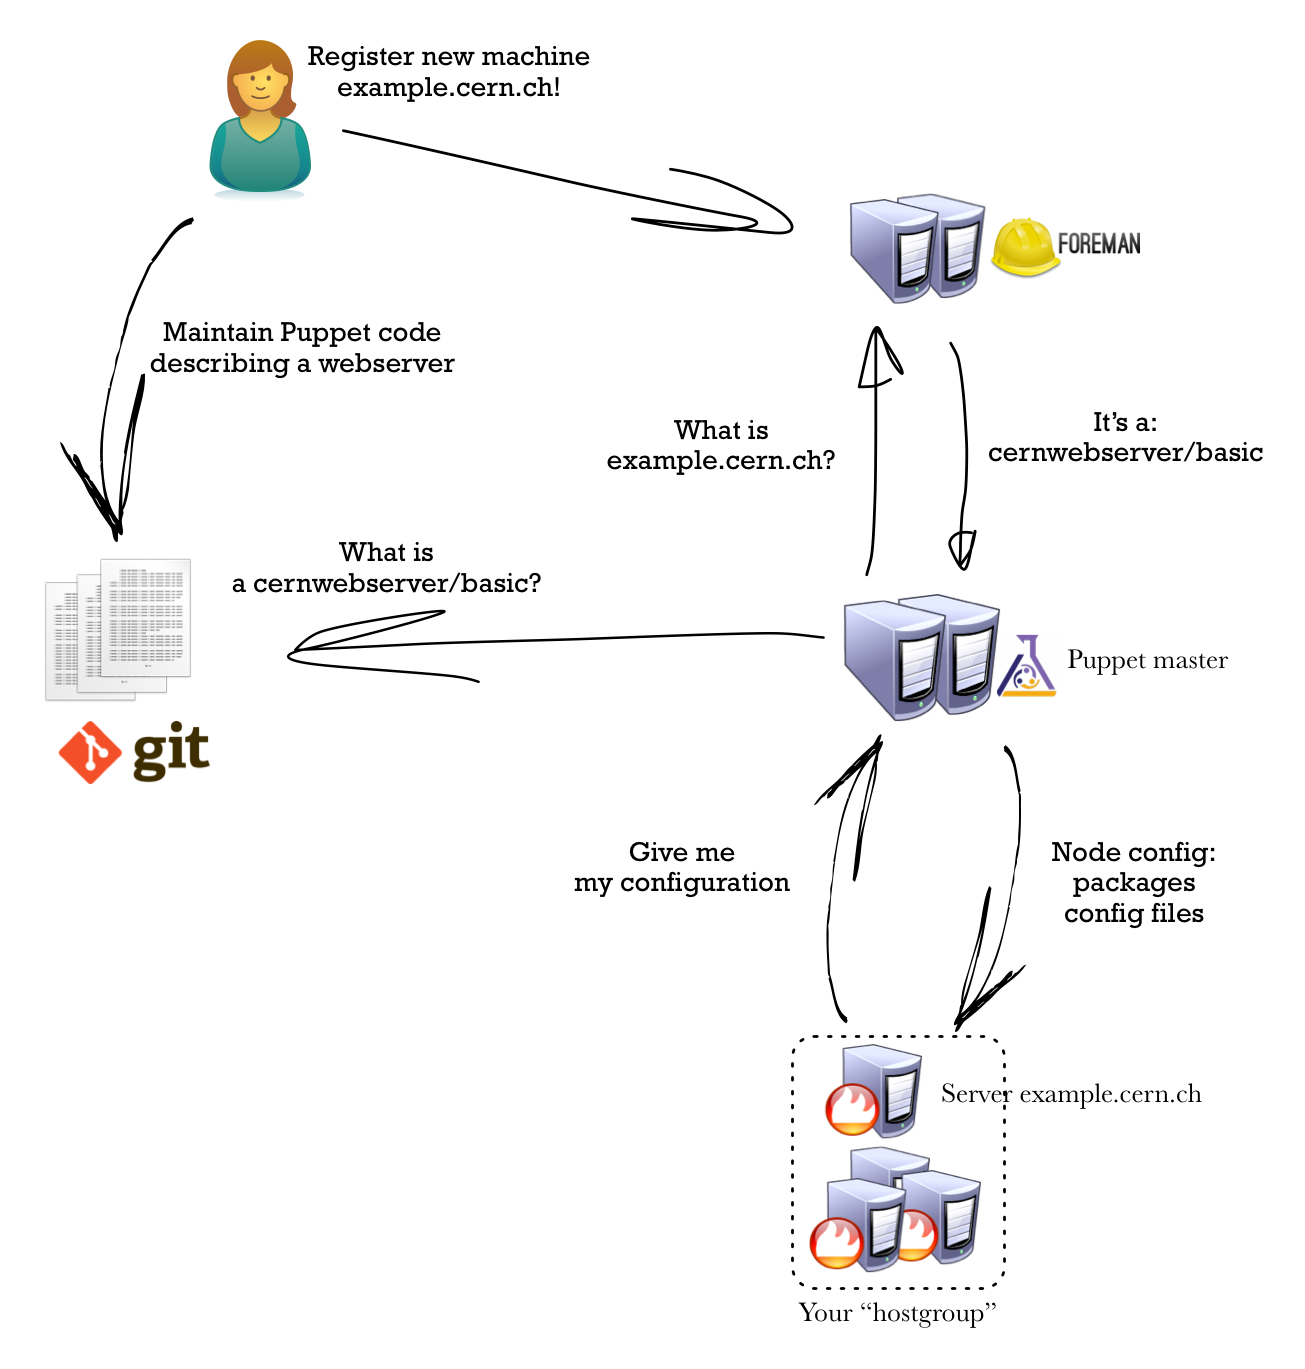
\includegraphics[width=\textwidth,height=\textheight,keepaspectratio]{ConfigurationManagement/PuppetRun/PuppetRun.png}
\caption{Puppet run interactions}
\end{figure}

\begin{enumerate}

\item When Puppet wants to run on the machine the local agent daemon asks
the Puppet master for its configuration. The Puppet master then queries
Foreman to get the node's hostgroup and environment.

\item Once the Puppet master knows the hostgroup and the environment of
the server it gets its manifest from a Git repository. This includes all
the modules linked to the manifest and eventually the Hiera variables.

\item At this point the Puppet master compiles the manifest and returns it
to the agent to apply it to the machine.

\item If the configuration provided by the master matches the actual one
then the agent does nothing, otherwise it makes the changes to reach the
desired configuration.

\end{enumerate}

This process is repeated automatically several time a day to ensure that
the server configuration stays the same all the time. Moreover a Puppet
run can be triggered manually using the agent's cli.

% TODO Expand with reports sent to Foreman and PuppetDb
